
\chapter{Related Work}
\label{ch:realted_work}

This chapter will give a brief introduction to neural networks and time delay neural networks, as well as an introduction to  automatic speech recognition with hidden Markov models. We also describe acoustic modelling using neural networks. These are the necessary building blocks for the work presented in this thesis.


\section{Neural Networks}
\label{sec:neural_networks}


TODO: Section about picking data, and tips like like data augmentation? 

In machine learning research, the goal of a \textit{neural network} is to approximate arbitrary functions. The basic idea of neural networks, so called \textit{perceptrons}, were first introduced by Rosenblatt in \cite{rosenblatt1958perceptron}. While the first neural networks were biologically motivated, neural networks can be interpreted as composition of functions. The relation between these functions forms a directed graph. In this work, we will only cover \textit{feed forward neural networks}. They are called feed forward neural networks because there are no feedback connections: The relation between all functions in the neural network forms an acyclic directed graph. Feed forward networks are an important building block for many machine learning applications. 
\\
More formally, as described in \cite{Goodfellow-et-al-2016}, a feed forward neural network can be described as a model $y = f^*(x, \theta)$, approximating an existing function $y = f(x)$. In this example $x$ is the input, $y$ is the output and $\theta$ are the model parameters which are learned during training. $f$ is the function to approximate and $f^*$ is a composition of many functions with the parameters $\theta$. 
\\
In practice, the functions composing a feed forward neural network are often simply chained, so that their relation graph simply forms a path. In this case, the functional components are called layers. A feed forward neural network of this form with $n$ layers can be written as follows:

\[
y = f^*_n \dots (f^*_2(f^*_1(x, \theta_1), \theta_2) \dots, \theta_n)
\]

For this type of neural network, $f^*_1$ is applied to the input, then $f^*_2$ is applied to the output of $f^*_1$, until the final layer is reached. The output of the final layer is the output of the neural network. Figure \ref{fig:simple_feed_forward_nn} shows a graph based representation of such a neural network. Each node represents a function, arrows represent data flows. 

\begin{minipage}{\linewidth}
	\makebox[\linewidth]{
	\begin{tikzpicture}[x=1.5cm, y=1.5cm, >=stealth]
	
	\node [every neuron] (n0) at (0*1-1,2.5-0) {$x$}; 
	\node [every neuron] (n1) at (1*1-1,2.5-0) {$f^*_1$}; 
	\node [every neuron] (n2) at (2*1-1,2.5-0) {$f^*_2$}; 
	\node [neuron hmissing] (n3) at (3*1-1,2.5-0) {}; 
	\node [every neuron] (n4) at (4*1-1,2.5-0) {$f^*_n$}; 
	\node [every neuron] (n5) at (5*1-1,2.5-0) {$y$}; 
	
	\draw [->] (n0) -- (n1);
	\draw [->] (n1) -- (n2);
	\draw [->] (n2) -- (n3);
	\draw [->] (n3) -- (n4);
	\draw [->] (n4) -- (n5);
	
	\end{tikzpicture}
	}
	\captionof{figure}{Simple graphical interpretation of feed forward neural network}
	\label{fig:simple_feed_forward_nn}
	\hspace{1cm}
\end{minipage}


Even with this simplification, it has been shown that such a feed forward neural network can approximate any function with any desired accuracy. This is called the \textit{universal approximation theorem}, the proof can be found in \cite{hornik1989multilayer}. The caveat is finding the correct function $f^*_n$ to use in each layer and the correct parameters $\theta_n$. Also, finding the function to approximate is non-trivial in the first place. We will discuss these problems in the next sections. 

\subsection{Training Neural Networks}

As with most machine learning approaches, we train the neural  network using by using a \textit{training dataset}, containing a lot of data points sampled from the distribution we seek to approximate. We usually do not want the neural network to excel on the training data set, but rather to perform well on unseen data. This ability is called \textit{generalization}. We can approximate the error on unseen data by testing the neural network on a \textit{test dataset}. The test dataset must never be used for adjusting the neural network parameters, as this will make the test dataset worthless. The situation where a network performs well on the training dataset but worse on the test dataset is called \textit{overfitting}. The network basically memorizes the distribution of the training dataset, but fails to generalize on the test dataset. \\
Given the definition in the past section, we can treat the problem of training a given neural network as finding appropriate parameters $\theta$ to minimize a certain \textit{error function} or \textit{loss function} $E = \mathcal{L}(y)$, where $E$ denotes the error and $y$ the network output. The error $E$ is usually some metric that judges the network performance based on the training data set. The state of the art algorithm for optimizing the parameters of a neural network is called \textit{stochastic gradient descend}, a special application of naive \textit{gradient descend}.
\subsubsection{Naive Gradient Descent}
\label{sec:gradient_descend}
To apply gradient descend, we have to calculate the derivative of the loss function, given a certain input, with respect to a certain parameter $\theta_i$. Since this derivative is multi-dimensional, it is called the \textit{gradient}. Given a feed forward neural network, we can write the error as follows:

\[
E = \mathcal{L}(f^*_n \dots (f^*_2(f^*_1(x, \theta_1), \theta_2) \dots, \theta_n))
\]

Thus, the derivative of the error with respect to a certain weight can be calculated by applying the chain rule.
\[
\frac{\partial E}{\partial \theta_i} = 
	\frac{\partial \mathcal{L}}{\partial y_n}
	\frac{\partial f^*_n}{\partial y_{n - 1}}
	\dots
	\frac{\partial f^*_{i + 2}}{\partial y_i}
	\frac{\partial f^*_i}{\partial \theta_i}
\]

Where $y_k$ is the result of $f^*_k$. \\
We know that the gradient $\frac{\delta E}{\delta \theta_i}$ will become zero in a local minimum, local maximum or saddle point of our error $E$. Since the gradient also gives the direction of the steepest slope, we can simply update our parameters iteratively, until we converge into a local minimum.

\[
	\theta_{i, t+1} = \theta_{i, t} - \epsilon * \frac{\delta E_{t}}{\delta \theta_{i, t}}
\]

In this equation, $t$ denotes the current time and the parameter $\epsilon$ is the so-called learning rate. $\epsilon$ has to be chosen by the designer of the neural network and influences not only the speed of convergence, but also whether the network converges at all. In literature, propagating the error gradient through a neural network is called \textit{backpropagation}. Backpropagation in the context of neural networks was first described in \cite{werbos1974beyond}.

\subsubsection{Stochastic Gradient Descend}

In practice, naive gradient descend does not work well, as described in \cite{wilson2003general}. The reason is that the function we seek to optimize when training a neural network is not convex and might have many local minima. Optimizing iteratively on a stationary error term makes this approach prone to falling into local minima. \\ \\
The state of the art algorithm for training neural networks is called \textit{stochastic gradient descent} (\textit{SGD}), which was first described in a context of neural networks in \cite{bottou1991stochastic}. Stochastic gradient descent introduces two fundamental changes and is. First, we no longer calculate our error term and corresponding gradient for the whole dataset, but for a randomly sampled subset of our data set, which is called a \textit{mini batch}, where the size of the mini batches is a design parameter. Second, we decrease our learning rate while training progresses. According to \cite{Goodfellow-et-al-2016}, iterating on mini batches adds noise to our error term, which in turn offers a regularization effect which was shown to lead to better generalization.
\\ \\
The noise introduced by stochastic gradient descend originates from the fact that we batch our dataset. Even if all batches, if averaged, represent the same distribution as our whole test dataset, each batch has a slightly different distribution. The shape of the loss function, and thus the gradient, changes slightly with each mini batch. This is the main reason why stochastic gradient descend is less prone to get stuck in local minima then naive gradient descend. The noise added by this stochastic process does not go away, even when we reach a global minimum. According to \cite{Goodfellow-et-al-2016}, this is be the main motivation for decreasing the learning rate over time. Furthermore, this property implies that the mini batch size is also an important design choice for achieving good generalization, not only for achieving fast training. 
\\ \\
A disadvantage of stochastic gradient descend is the slower convergence, since we need more steps. This is remedied by the fact that it is easier to calculate the gradient for a small mini batch instead of the whole dataset at once. In practice, we usually shuffle our dataset, split it into mini-batches, and then process each mini batch once. An iteration over all mini batches in the dataset is called an \textit{epoch}. 

\subsubsection{Learning Rates and Learning Rate Scheduling}

With stochastic gradient descend, we choose a separate learning rate $\epsilon_k$ for each epoch $k$. In the scope of this work, we only introduce \textit{exponential decay}, a very simple scheduling algorithm for the learning rate, although numerous other schedulers exist. \\
Exponential starts with a learning rate $k_0$ for the initial batch and multiplies the learning rate by a factor of $0 < p < 1$ after each epoch. 
\[
k_n = k_{n - 1} * p
\]
A variant of exponential decay keeps the learning rate constant for a number epochs, until the improvement of error measured on the test dataset falls below a certain threshold $t$. This variant is called \textit{newbob}. Newbob scheduling is widely used by the speech recognition community. It was first introduced in \cite{berkely2000newbob}.

\subsubsection{Momentum}

\textit{Momentum} is another technique that was shown to avoid local minima. When using momentum, we do not apply the gradient directly to our model, but rather use a linear combination of the gradient of the last batches. There are multiple versions to achieve momentum when using stochastic gradient descend. This work uses the notation introduced in \ref{polyak1964some} and throughly analyzed in the context of deep learning in \ref{sutskever2013importance}:
\begin{align*}
\upsilon_{i, t+1} &= \upsilon_{i, t} * \rho + \epsilon * \frac{\delta E_{t}}{\delta \theta_{i, t}} \\
\theta_{i, t+1} &= \theta_{i, t} - \upsilon_{i, t+1}
\end{align*}
Here, $\upsilon$ is called the \textit{velocity}, it is a linear combination of the last velocity and the current gradient. $\rho$ is the term defining the momentum. It defines how much of the velocity is added to the current gradient. All other variables are defined as in section \ref{sec:gradient_descend}.

\subsection{Neural Network Architectures}

In practice, neural network layers are often formed by combining an affine transformation with a non-linear function. Since affine transformations of data vectors can be interpreted as matrix-vector multiplications, we can write a layer function in the following way, where $x_k$ is the input vector for $k$th layer, $W_k$ is the matrix defining the affine transformation of the $k$th layer, and $\varphi$ is a non-linear activation function of layer $k$.
\[
f^*_k(x_k) = \varphi_k(W_k x_k)  
\]
The count of layers, as well as the size of each $W_k$ are design decisions and depend on the task. We call the count of layers \textit{depth} of a neural network, and count of rows in $W_k$ the \textit{width} of layer $k$. The contents of $W_k$, called the \textit{weights} of layer $k$, are the trainable parameters $\theta$ for models of this form.
\pagebreak
\subsubsection{Activation Functions}

Non-linear activation functions, or simply \textit{activation functions}, can be roughly classified into two groups: Activation functions which are applied element-wise and thus do not change the dimension of the data, as well as activation functions which are applied on groups of elements of the input vector and change the dimension. The latter case is commonly fund with so called pooling functions. The choice of the activation function $\varphi$ has significant impact on the performance of a neural network and has been subject to many bodies of research, as summarized in \cite{thoma2017analysis}. In this work, we will only discuss the \textit{ReLU}, \textit{p-norm} and \textit{softmax} activation functions. 

\subsubsection*{Rectified Linear Unit (ReLU)}
% ReLU
\begin{minipage}{0.45\textwidth}
	\[\varphi^{ReLU}(x) = \begin{cases}
	0 & x < 0 \\
	x & x \geq 0
	\end{cases}\]
	First introduced in \cite{krizhevsky2012imagenet}, ReLU nonlinearities have proven successful in practice. The computation of ReLU nonlinearity is cheap, also the gradient never saturates for positive values of $x$. For negative values, the gradient is zero, which can be a disadvantage.  
\end{minipage}
\hfill
\begin{minipage}{0.45\textwidth}
\begin{tikzpicture}[baseline=(current bounding box)]
\begin{axis}[xmin=-2,xmax=2,ymin=-2,ymax=2,axis lines = middle,xlabel = $x$,ylabel = $\varphi^{ReLu}(x)$,clip = false]
\addplot+[mark=none,blue,domain=-2:0] {0};
\addplot+[mark=none,blue,domain=0:2] {x};
\end{axis}
\end{tikzpicture} 
\captionof{figure}{The ReLU function.}
\end{minipage}
% L2 Pooling

\subsubsection*{P-norm}
\begin{minipage}{0.45\textwidth}
	\[\varphi^{Lp}(X) = \sqrt[p]{ \sum_{x \in X}{x^p} } \] 
	The p-norm nonlinearity was described by \cite{zhang2014improving}. This nonlinearity operates on a set $X$ of input elements and reduces them to one. The group size as well as the $p$ are a design parameter. For a fixed $p$ of $2$, the p-norm is also called \text{L2 pooling}.
\end{minipage}
\hfill
\begin{minipage}{0.45\textwidth}
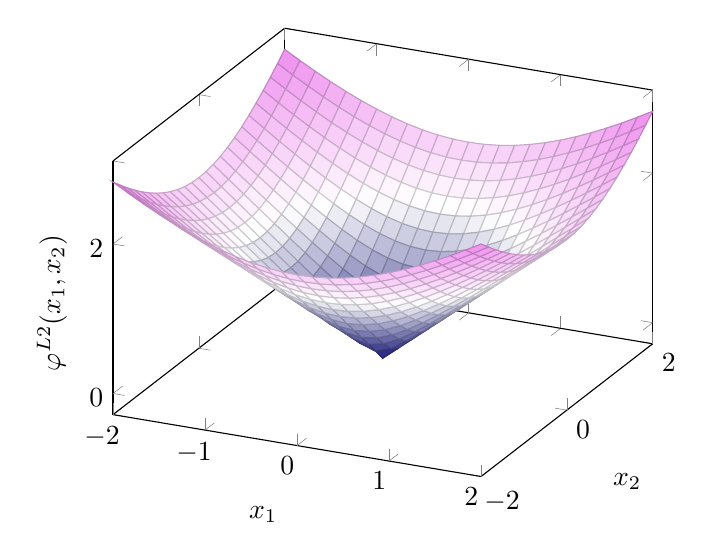
\begin{tikzpicture}[baseline=(current bounding box)]
\begin{axis}[xmin=-2,xmax=2,ymin=-2,ymax=2,xlabel = $x_1$,ylabel = $x_2$,zlabel = $\varphi^{L2}({x_1, x_2})$,colormap/violet,clip = false]
\addplot3[surf,samples=25, domain=-2:2]
{sqrt(x * x + y * y)};
\end{axis}
\end{tikzpicture}
\captionof{figure}{Example of p-norm with $p = 2$ and and an input group containing two values}
\end{minipage}

\subsubsection*{Softmax}
\begin{minipage}{0.45\textwidth}
	\[\varphi^{softmax}_{\tau}(X)_i = \frac{e^\frac{x_i}{\tau}}{ \sum_{x_j \in X} e^\frac{x_j}{\tau} } \]
	The softmax activation is defined as an operation over the whole input, but does not reduce the dimension. It maps all output values to a space between $0$ and $1$, preserves the rank of each output and also guarantees that the sum over all outputs is exactly $1$. Therefore it produces a valid probability distribution and is usually used for the last layer of a neural network for classification problems. The term $\tau$ is called the softmax temperature. It can be used to change the contrast of the distribution produced by the softmax activation. A higher temperature $\tau$ will lead to a distribution more smooth. A lower $\tau$ will lead to a more sharp distribution, that concentrates a higher probability at the maximum value. 
\end{minipage}
\hfill
\begin{minipage}{0.45\textwidth}
	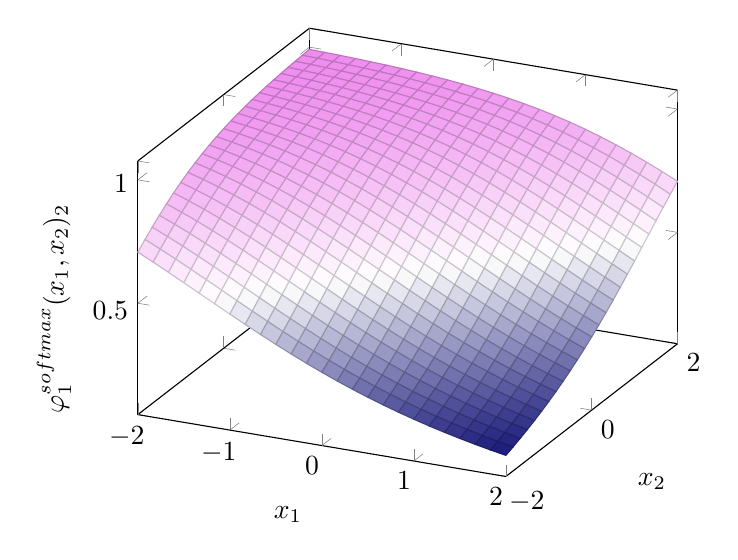
\begin{tikzpicture}[baseline=(current bounding box)]
	\begin{axis}[xmin=-2,xmax=2,ymin=-2,ymax=2,xlabel = $x_1$,ylabel = $x_2$,zlabel = $\varphi^{softmax}_{1}({x_1, x_2})_2$,colormap/violet,clip = false]
	\addplot3[surf,samples=25, domain=-2:2]
	{sqrt(e^y / (e^x + e^y) )};
	\end{axis}
	\end{tikzpicture}
	\captionof{figure}{Example of a vanilla softmax ($\tau = 1$) for an input vector containing two values}
	\vspace{0.5cm}
	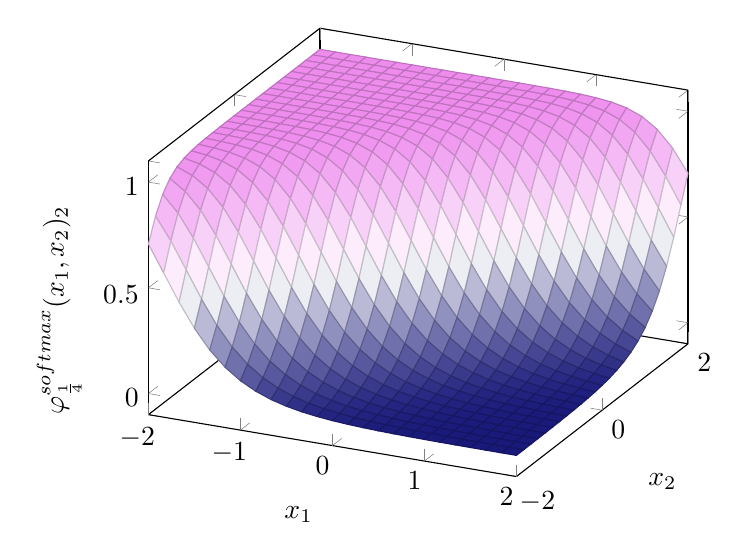
\begin{tikzpicture}[baseline=(current bounding box)]
	\begin{axis}[xmin=-2,xmax=2,ymin=-2,ymax=2,xlabel = $x_1$,ylabel = $x_2$,zlabel = $\varphi^{softmax}_{\frac{1}{4}}({x_1, x_2})_2$,colormap/violet,clip = false]
	\addplot3[surf,samples=25, domain=-2:2]
	{sqrt(e^(y * 4) / (e^(x * 4) + e^(y * 4)) )};
	\end{axis}
	\end{tikzpicture}
	\captionof{figure}{Example of a softmax with adjusted temperature ($\tau = \frac{1}{4}$) for an input vector containing two values}
\end{minipage}

\subsection{The Cross Entropy Loss Function}

There exist numerous loss functions for neural networks. Technically, any metric can be used as loss function, although loss functions do not necessarily have to be metrics. One of the most widely loss functions for classification tasks is the \textit{cross entropy} (\textit{CE}) function. For two  probability vectors $p$ and $q$, the cross entropy can be written as follows:

\begin{align}
H(p, q) = - \sum_{x} p(x) \log q(x)
\label{eq:cross_entropy_loss}
\end{align}

The cross entropy loss function has several important properties. First, it minimizes the so called \textit{Kullback-Leibler} (\textit{KL}) divergence. The Kullback-Leibler divergence measures the distance of two probability distributions and was introduced in \cite{kullback1951information}. The Kullback-Leibler divergence is equal to zero if, and only if, the two given distributions are also equal. For two probability vectors $p$ and $q$, it can be written in the following way:

\[
D_{KL}(p, q) = -\sum_{x} p(x) \log \frac{p(x)}{q(x)}
\]

To show the connection between the cross entropy and the Kullback-Leibler divergence, we first assume that $q$ is the distribution we seek to optimize. Thus $p$ can be thought of as an example from our training dataset, or in other words, the distribution we seek to match. Therefore, $p$, can be assumed to be constant. We can write the Kullback-Leibler divergence as follows: 

\begin{align*}
D_{KL}(p, q) &= - \sum_{x} p(x) \left[ \log p(x) - \log q(x) \right] \\
& = - \sum_{x} p(x) \log p(x) -\sum_{x} p(x) \log q(x)
\end{align*}

Since we are not interested minimizing the distribution $p$, we can drop the first sum, and thus receive the cross entropy loss as in equation \ref{eq:cross_entropy_loss}. 
\subsection{Cross Entropy Loss for Classification}
\label{sec:ce_loss}
When training neural networks, we often deal with classification problems. In this case, we seek to assign a single class to a given input sample, our target probability $p$ has exactly one element which is one, all other elements are zero. In this case, the cross entropy loss can be simplified to the so called \textit{negative log likelihood loss}, where $i$ is the index of the correct class in $p$. 

\begin{align}
D_{NLLL}(i, q) = -\log q(i)
\label{eq:nlll}
\end{align}

It has to be noted that this loss functions all operate on probability vectors: All elements have to be between $0$ and $1$ and sum to unity. Therefore, a softmax activation function is usually applied before calculating the loss. \\ \\
It can further be shown that training using a cross entropy loss function trains the network to predict \textit{posteriori} probabilities \cite{richard1991neural}. Formally, given an network input $x$ and a class $c_i$, the network will predict $p(c_i|x)$. Since posteriors are inherently biased towards more frequent classes, we might want to estimate the likelihood $p(x|c_i)$ instead, depending on our use case. With bayes' theorem, we can write the posterior depending on the likelihood. 
\[
p(c_i|x) = \frac{p(x|c_i) p(c_i)}{p(x)}
\]
We now assume $p(x)$ to be equal for all $x$ and solve the equation for the likelihood:
\[
p(x|c_i) = \frac{p(c_i|x)}{p(c_i)}
\]
The probability of observing a certain class $p(c_i)$ is called a \textit{prior}. The prior can be estimated from the training data, or from the network output given a random sample of the training data set. Using the likelihood instead of the prior is especially important when the examples in the training set are highly unbalanced with regard of one or more classes. 


\section{Time Delay Neural Networks}
\label{sec:tdnn}

\textit{Time delay neural networks} were introduced by Waibel et. al in \cite{waibel1990phoneme}. The purpose time delay neural networks is to model long time dependencies in a robust way. The central idea behind this network type is to use several time frames of input, and to not use fully-connected layers, but rather layers that impose temporal structure. \\ \\
To achieve this, the network not only receives the current frame $x_{0,t}$ as input, but also the $n$ previous frames $x_{0,t - 1}, ..., x_{0,t - n}$ as input. These frames are delayed in time, hence the name. Then, the a weighted sum is applied to the input, where the weights are learned parameters. This is called a \textit{TDNN unit} or \textit{TDNN layer} with a filter kernel of size $n$. TDNN layers can be stacked. If this is the case, preceding layers have to be extended to produce an output that contains multiple time frames. \\
Formally, we can write for $x_{k,t}$, the output of the $k$-th TDNN layer at time t for the feature vectors with size one:
\[
x_{k,t} = \sum_{i = 1}^n w_{k, i} x_{k - 1, t - i}
\]
Where $w_{k, i}$ is denotes the $i$-th weight of the weighted sum used by the $k$-th layer. \\
This equation can be rewritten using a discrete convolution operator. In this case $w_k$ is called a convolution kernel. 
\[
x_{k} = w_{k} * x_{k - 1}
\]
For feature vectors containing more than one feature, we introduce the concept of \textit{channels}. A channel can be considered a dimension in the feature. We can write this case for $p$ input channels and $q$ output channels, where $w_{k, j}$ is now a multi-dimensional kernel, producing the output channel $j$. Each TDNN layer will learn $q$ such kernels, while each kernel is large enough to take all $p$ input channels into account. 
\[
x_{k,j} = w_{k, j} * x_{k - 1}
\]
The concept of interpreting TDNN layers as convolutions is not new, but very useful. The generalization to multi-dimensional convolutions is called \textit{convolutional neural networks} and was shown to be incredibly successful \cite{krizhevsky2012imagenet}. Since TDNNs only apply the convolution over the time dimensions, it can be useful to interpret a TDNN as a so called \textit{finite impulse response} (\textit{FIR}) filter. As described in \cite{leon2015signale}, finite impulse response filters are inherently stable, as they the output is always a sum of finite elements. They also do not accumulate rounding errors. \\
In \cite{waibel1990phoneme}, another interesting property is given: Since there are a lot less learned parameters than operations, a TDNN layer is forced to only focus on the most important features in the data, which leads to better generalization. This so-called \textit{parameter sharing} is achieved by averaging gradients of all operations for their respective weight, independently of the time context $t$. According to \cite{Goodfellow-et-al-2016}, this is one of the main reasons of success for convolutional neural networks in general. 

\subsection{Pooling, Stride and Splicing}

It should be noted that most successful convolutional architectures, as \cite{krizhevsky2012imagenet}, combine convolutional layers with pooling nonlinearities. This is done because pooling over the layer output enables to network to learn several different representations of the same concept, where the pooling will forward the most dominant to the next layer. \\
Furthermore, it was shown that using larger steps in the convolution operation can lead to better results \textit{springenberg2014striving}. In the context of TDNNs, this means that we would not use adjacent frames for concatenating our input, but frames which are further apart. In literature, this is called \textit{stride} or \textit{strided convolution}, where the the stride $s$ gives the distance between concatenated frame. For a strided convolution, the input vector can be written as:
\[
x_{0,t}, x_{0,t + s}, ..., x_{0,t + ns}
\] 
It is also possible to define a list of indexes $S = (s_1, ..., s_n)$ to concatenate, which is especially useful if the distance between concatenated frames should not be uniform. This operation is called \textit{splicing} and was introduced by \cite{peddinti2015jhu}. In this case, our input vector becomes: 
\[
x_{0,ts_1}, x_{0,t + s_2}, ..., x_{0,t + s_n}
\] 

\subsection{A visual Example}

TDNNs allow a straight-forward interpretation of their layer outputs as multi-dimensional signals, which makes visualization over time helpful. We want to conclude this section with the visualization of a tiny TDNN that was trained to distinguish $53$ phones in an audio sample. We use $40$ log-mel coefficients as features. Log-mel coefficients are introduced in section \ref{sec:lmel}. \\ \\
Figure \ref{fig:tiny_tdnn} shows our tiny TDNN model in the time domain. Our input vector has $40$ channels and a time context of $21$. The first TDNN layer uses $40$ filter kernels of size $5*40$ and a stride of $4$. It and is followed by an L2 norm with group size $2$, resulting in a layer output with $5$ time frames and $20$ channels. The second TDNN layer uses $40$ filter kernels of size $5*20$ and a stride of $5$. It is followed by an L2 norm with group size $2$, resulting in an output spanning $1$ time frame and $20$ channels. In the end, we apply a linear layer that maps the $20$ channels to $53$ phone classes, including special classes for silence and noise.\\
\begin{minipage}{\linewidth}
	\vspace{5mm}
	\begin{tikzpicture}[x=1.8cm, y=1.5cm]
	% Layers
	\node[text width=3cm] at (-1,0) {Input ($21*40$)};
	\foreach \m in {2,3,...,20}
	\node [tdnn neuron] (input-\m) at (\m*0.25,0) {};
	
	\node [tdnn neuron, label=below:$x_{t - 10}$] (input-1) at (1*0.25,0) {};
	\node [tdnn neuron, label=below:$x_{t + 10}$] (input-21) at (21*0.25,0) {};
	
	\node[text width=3cm] at (-1,0.5) {TDNN/LP 1};
	\node[text width=3cm] at (-1,1) {Hidden ($5*8$)};
	\foreach \m [count=\y] in {1,2,...,5}
	\node [tdnn neuron] (hidden-1-\m) at (\y*0.25*4 - 0.25,1) {};
	
	\node[text width=3cm] at (-1,1.5) {TDNN/LP 2};
	\node[text width=3cm] at (-1,2) {Output ($1*6$)};
	\node [tdnn neuron, label=above:$y_{t}$] (classify-1) at (1*0.25 + 10 * 0.25,2) {};
	
	%Edges
	\foreach \m [
	evaluate=\m as \nstart using int(((\m - 1) * 4) + 1),
	evaluate=\m as \nstep using int(((\m - 1) * 4) + 2),
	evaluate=\m as \nend using int(((\m - 1)* 4) + 5)] in {1,2,...,5}
	\foreach \i in {\nstart,\nstep,...,\nend}
	\draw (input-\i.north) -- (hidden-1-\m); % Error happens here. 
	
	\foreach \m in {1,2,...,5}
	\draw (hidden-1-\m) -- (classify-1);
		
	\end{tikzpicture}
	\captionof{figure}{Tiny TDNN model}
	\label{fig:tiny_tdnn}
	\vspace{5mm}
\end{minipage}

We trained this tiny TDNN model on $14$ hours of voice data using the newbob-learning rate scheduler. Figures \ref{fig:tiny_tdnn_1_weights}, \ref{fig:tiny_tdnn_2_weights} and \ref{fig:tiny_classifier_weights} show the learned filter kernels and weights after training. Warmer colors indicate higher values, the horizontal axis corresponds to time, while the vertical axis corresponds to channels. For the first TDNN layer, it can be seen that filters which are in the same pooling group learn similar parameters. For the other layers, the filters are harder to implement, as TDNN layers do not preserve the ordering of channels. They are still shown for completeness. \\
\noindent
\weightillustration
	{images/tdnn_example/large_weight_tdnn_1.png}
	{$40$ learned filters of TDNN layer $1$}
	{fig:tiny_tdnn_1_weights}
\weightillustration
	{images/tdnn_example/large_weight_tdnn_2.png}
	{$24$ learned filters of TDNN layer $2$}
	{fig:tiny_tdnn_2_weights}
\smallweightillustration
	{images/tdnn_example/large_weight_classifier.png}
	{Affine transformation learned by the final linear layer}
	{fig:tiny_classifier_weights}

We now visualize the outputs of different layers given an audio sample of a few seconds length. Figures \ref{fig:tiny_input_signal} to \ref{fig:tiny_softmax_out} show the output of the TDNN and LP layers, as well as the output after the linear and the softmax layer. Such layer outputs are also called \textit{activations}. The audio sample is shown in Figure \ref{fig:tiny_input_signal} and originates from a female speaker saying \textit{``And these are always periods, ladies and gentlemen, accompanied by turbulence.''}.

\noindent
\weightillustration
	{images/tdnn_example/large_0_input.png}
	{Input features extracted from the audio sample}
	{fig:tiny_input_signal}
\weightillustration
	{images/tdnn_example/large_1_tdnn_1.png}
	{Output of the first TDNN layer}
	{fig:tiny_tdnn_1_out}
\weightillustration
	{images/tdnn_example/large_4_lp_1.png}
	{Output of the first L2 pooling layer}
	{fig:tiny_lp_1_out}
\weightillustration
	{images/tdnn_example/large_5_tdnn_2.png}
	{Output of the second TDNN layer}
	{fig:tiny_tdnn_2_out}
\weightillustration
	{images/tdnn_example/large_8_lp_2.png}
	{Output of the second L2 pooling layer}
	{fig:tiny_lp_2_out}
\weightillustration
	{images/tdnn_example/large_10_classifier.png}
	{Output of the linear layer}
	{fig:tiny_classifier_out}
\weightillustration
	{images/tdnn_example/large_11_softmax.png}
	{Output of the softmax layer, the final network output}
	{fig:tiny_softmax_out}


%24: PaddyAshdown_2011X\PaddyAshdown_2011X_71_6: and these are always periods ladies and gentlemen accompanied by turbulence


\section{Automated Speech Recognition}
\label{ch:HMM_ASR}
\textit{Automated speech recognition} (\textit{ASR}) is the task of generating a text transcription from a given sample of spoken language using a computer system. In literature, this problem is also referred to as \textit{speech to text} (\textit{SST}). \\
Many approaches exist for solving this task. In this work, we will focus on automated speech recognition using systems that are based on hidden markov models. The contents of this this section, except otherwise noted, is based upon the lecture Automated Speech Recognition of Karlsruhe Institute of Technology \cite{kitasr2018stueker}, which is in turn based on the books \cite{schukat1995automatische} and \cite{huang2001spoken}. \\ \\
Automated speech recognition systems usually follows an architecture that separates \textit{preprocessing} of the audio signal and \textit{decoding}. The preprocessing transforms a brief time window of the audio signal into a feature vector. The decoding uses a statistical model assembled from an \textit{acoustic model}, a \textit{dictionary} and a \textit{language model} to calculate the most likely text representation, given the feature vectors.\\ \\

More formally, we can treat the decoding as a classification problem. Let $a$ be a set of feature vectors, we seek to find the word sequence $w^*$ that was most likely for $a$ under our model. That can formally be written as follows, where $p(w|a)$ is the conditional probability of event $w$ given $a$:

\[
w^* = \underset{w}{\arg \max} \; P(w|a)
\] 
We do not know $P(w|a)$, but can re-write it using Bayes' theorem:

\[
w^* = \underset{w}{\arg \max} \; \frac{P(a|w) P(w)}{P(a)}
\]

Since $p(a)$ is the same for all possible word sequences $w$, we can drop the denominator from this equation:

\begin{align}
w^* = \underset{w}{\arg \max} \; P(a|w) P(w)
\label{eq:asr_base_formula}
\end{align}

Equation \ref{eq:asr_base_formula} is called the \textit{fundamental equation of automated speech recognition}. While the fundamental equation seems straight forward, the difficult task is to create a reliable and computationally tractable model for approximating the probability of an acoustic feature given a word sequence, $p(a|w)$ and the probability of observing a word sequence $p(w)$. Finding $p(a|w)$ is the purpose of the acoustic model. The language model is responsible for finding $p(w)$. 

\subsection{Preprocessing}
Preprocessing, also called the \textit{frontend}, transforms some audio signal into a sequence of feature vectors. To do so, we sample an audio signal using a microphone, then the signal is windowed and the frequency spectrum is calculated for each window of the signal. This process is called short time fourier transform, as defined in section \ref{sec:reverberation}, equation \ref{eq:stft}. Hence, the resulting spectral coefficients are also often called \textit{fourier coefficients}. It should be noted that there are more sophisticated approaches to extract the frequency components of a windowed signal, notably the \textit{continous wavelet transform}, as described in \cite{mallat1999wavelet}, which has better properties in terms of time and frequency resolution. \\ \\
There exist numerous approaches to transform the spectrum of a signal to useful features. In this work, we only discuss so called \textit{log-mel coefficients}. 
\subsubsection{Log-Mel Coefficients}
\label{sec:lmel}
Log-mel coefficients were introduced in \cite{waibel1990phoneme} and \cite{waibel1983comparative}. This approach is physiologically motivated: Similar to human hearing, the mel-scale provides a better relative frequency resolution in lower frequencies \cite{waibel1990phoneme}. \\
As given in \cite{poser1990speech}, the mel-scale is defined by the following relation to the regular frequency spectrum in Hertz: 
\[
MEL(f)=2595\log _{10}\left(1+{\frac {f}{700}}\right)
\]
Very often, the number of coefficients is reduced to get smaller feature vectors $(\sigma_1, ..., \sigma_n)$. This is done by summing all coefficients in certain windows $\sigma_k$ on the mel-scale: 
\[
MEL_k = \int \sigma_k(f) * MEL(f) \delta f 
\]

Usually a triangle window is used. In literature, the weighted sum is also referred to as \textit{filter bank} \cite{zhan1997vocal}. \\
The $k$-th log-mel coefficient is then calculated by applying a logarithm:
\[
lMEL_k = \log(MEL_k) 
\]
A graphical example of log-mel coefficients can be seen in figure \ref{fig:tiny_input_signal}.
\\ \\
In literature, \textit{Mel-Frequency-Cepstral-Coefficients} (\textit{MFCCs}) are frequently mentioned. They are not to be confused with log-mel coefficients. MFCCs can be calculated by applying an inverse discrete cosine transform on the the log-mel coefficients \cite{davis1990comparison}.

% Our experiments use VTLN with a warp factor of 1.0. According to the janus implementation, that does not do anything. 
%\subsubsection{Vocal Tract Length Normalization}
%TODO: 
%https://www.lti.cs.cmu.edu/sites/default/files/CMU-LTI-97-150-T.pdf

\subsection{Acoustic Model}
\label{sec:acoustic_model}
The acoustic model $A$ is responsible of giving us the likelihood of observing a certain word sequence $W$, for a given sequence of features $X$. 
\[
	P(X|W)
\]
Since language does not have one fixed speed, but can rather be slow or fast, acoustic models usually make use of hidden markov models combined with some discriminative classification approach. The discriminative classifier is responsible for predicting the observation probability for a certain symbol of the hidden markov model. The most prominent classifier for this specific task is the gaussian mixture models, which combines several normal distributions to approximate a more complex distribution. The parameters of the acoustic model are usually learned using the Baum-Welch equations introduced in the previous section. \\ \\
Before we explain the architecture of the hidden markov model model used for the acoustic model, we have to introduce the linguistic concepts of \textit{phonemes}, \textit{phones} and \textit{allophones}. Phonemes are sound atoms in a spoken language, that are relevant for the meaning of a spoken word. In other words, if a phoneme in a spoken word changes, the meaning of this word would change. Allophones are different pronunciation version of the same phoneme. \textit{Phones} are simply distinct sounds that are found in a language, regardless of whether swapping a phone changes the meaning of the word or not. \\ \\
In the case relevant for this work, the acoustic model models so called context dependent sub-phones, which are then combined into words or word sequences using the dictionary. Sometimes, allophones are modeled as well, to capture variants. For simplicity we will also refer to allophones as phones. \\
Context dependent phones include predecessor and successor phones into their model. This happens by introducing extra hidden HMM states for $n$-tupels of phones. These context-dependent phones are then called \textit{diphones}, \textit{triphones} or \textit{quinphones}. This approach leads to a very high number of HMM quickly, so context-dependent phones have to be chosen carefully. \\
For modeling so-called sub-phones, the model distinguishes between start, middle, and end part of an phone as three distinct hidden markov model states, which represent the phone together. This has the advantage of introducing some speed invariance into the model: It does no longer matter whether a certain phone was spoken very slowly or fast. Figure \ref{fig:sub_three_allophone} shows a hidden markov model for such an approach. \\
\begin{minipage}{\linewidth}
	\makebox[\linewidth]{
		\begin{tikzpicture}[x=1.5cm, y=1.5cm, >=stealth]
		
		\node[state] (s1) at (0,1) {$a_s$}
		edge [loop above] ();
		\node[state] (s2) at (3,1) {$a_m$}
		edge [<-,bend right=45] (s1)
		edge [loop above] ();
		\node[state] (s3) at (6,1) {$a_e$}
		edge [<-,bend right=45] (s2)
		edge [loop above] ();
		% observations
		\node[observation] (v1) at (0,0) {$a_s$}
		edge [lightedge] (s1);
		\node[observation] (v2) at (3,0) {$a_m$}
		edge [lightedge] (s2);	
		\node[observation] (v3) at (6,0) {$a_e$}
		edge [lightedge] (s3);
		
		\end{tikzpicture}
	}
	\captionof{figure}{Hidden markov model for a phone model with three sub-states for start $a_s$, middle $a_m$ and end $a_e$}
	\label{fig:sub_three_allophone}
	\hspace{1cm}
\end{minipage}
A single HMM state in such a model is also referred to as \textit{distribution} or \textit{senone} for historical reasons \cite{yu2016automatic}.
\subsection{Dictionary}
\label{sec:dictionary}
The purpose of the dictionary is to describe the pronunciation of words in terms of phones. The dictionary is usually given. A common way to create a dictionary is to generate it using a set of rules and a list of words, and then fine-tune it by hand. The dictionary also contains different pronunciation variants for each word. 

\begin{minipage}{\linewidth}
	\makebox[\linewidth]{
		\begin{tikzpicture}[x=1.5cm, y=1.5cm, >=stealth]
		
		\node[state] (AX) at (0,0) {\textscripta };
		\node[state] (EH) at (0,1) {\textipa{E}};
		\node[state] (IX) at (0,2) {\textbari };
		
		\node[state] (N) at (1,1) {\textipa{n}}
		edge [<-,bend right=15] (AX)
		edge [<-] (EH)
		edge [<-,bend right=-15] (IX);
		\node[state] (EY) at (2,1) {\textipa{e}\textsci }
		edge [<-,bend right=45] (N);
		\node[state] (B) at (3,1) {\textipa{b}}
		edge [<-,bend right=45] (EY);
		
		\node[state] (AX2) at (4,1) {\textscripta }
		edge [<-,bend right=45] (B);
		\node[state] (L) at (5,1) {\textipa{l}}
		edge [<-,bend right=-45] (B)
		edge [<-,bend right=45] (AX2);
		\node[state] (AXR) at (6,1) {\textrhookschwa }
		edge [<-,bend right=45] (L);
		\end{tikzpicture}
	}
	\captionof{figure}{Markov chain for pronunciation variants of the word \textit{enabler}, where the state names correspond to their respective IPA phones}
	\label{fig:dictionary_hmm}
	\hspace{1cm}
\end{minipage}
Figure \ref{fig:dictionary_hmm} shows such a model for a single word. Emissions are not shown, as each state in this model refers the hidden markov model associated with the corresponding phoneme. Transitions that are not modeled in the dictionary are constant zero, also the dictionary contains no trainable parameters.
 
\subsection{Language Model}
\label{sec:language_model}
In the fundamental formula of speech recognition, the language model gives the probability of a word sequence. Practically, the language model gives the probability of a word following a certain sequence of words. Since languages tend to have many words, calculating the transmission probability for each given word pair would be intractable. Instead of this, so called $n$-gram language models can be used. $n$-gram language models count the occurrence of word tuples of length $n$ in a large text corpora. The occurrences are then used to calculate the probability of a word $w_i$, given $n - 1$ predecessors $w_{i - 1}, ..., w_{i - n}$.

\[
P(w_i|w_{i - 1},...,w_{i - n})
\]

For a $2$-gram model, the transition probabilities can be directly derived by norming the count of occurrences for each successor. An example for such a model is shown in figure \ref{fig:lm_hmm}. For larger $n$, we have a state for each feasible combination of words, which quickly becomes intractable. \\ 
\begin{minipage}{\linewidth}
	\makebox[\linewidth]{
		\begin{tikzpicture}[x=1.5cm, y=1.5cm, >=stealth]
		
		\node[state,minimum size=1cm] (that) at (2,0) {that}
		edge [loop below] node[auto] {$\frac{1}{2}$} ();
		\node[state,minimum size=1cm] (is) at (0,3) {is}
		edge [<-,bend right=15] node[auto, swap] {$\frac{1}{4}$} (that)
		edge [->,bend right=-15] node[auto] {$\frac{1}{4}$} (that)
		edge [loop above] node[auto] {$\frac{1}{4}$} ();
		\node[state,minimum size=1cm] (not) at (4,3) {not}
		edge [<-,bend right=-15] node[auto] {$0$} (that)
		edge [<-,bend right=15] node[auto,swap] {$\frac{1}{2}$} (is)
		edge [->,bend right=15] node[auto, swap] {$0$} (that)
		edge [->,bend right=-15] node[auto] {$1$} (is)
		edge [loop above] node[auto] {$0$} ();
		\end{tikzpicture}
	}
	\captionof{figure}{Markov chain built from a $2$-gram language model for the sentence \textit{``That that is, is; that that is not, is not."}, omitting start and end literals}
	\label{fig:lm_hmm}
	\hspace{1cm}
\end{minipage}
It should be noted that other approaches for language modeling exist, most notably recurrent neural network based language models \cite{mikolov2011extensions}. 
\subsection{Decoding Process}
The decoding step combines the acoustic model, dictionary, and language model to find the text for a given observed utterance. This section describes decoding in a very fundamental way. In real-world applications, many more details are considered. \cite{huang2001spoken} and \cite{yu2016automatic} give a very detailed description of different decoding approaches.\\
It is possible decompose any word sequence $W$ into a number possible sequences of HMM states using the introduced HMM based acoustic model and the dictionary. Let $Q = (s_1, ..., s_n)$ be such a HMM state sequence. We can approximate the fundamental formula of speech recognition in the following way: 
\begin{align}
W^* &= \underset{W}{\arg \max} \; P(W) \; \underset{Q}{\max} \; P(X|Q)
\label{eq:viterbi_assumption}
\end{align}
This formulation is called the \textit{viterbi approximation} \cite{huang2001spoken}. With it finding the probability for a certain word sequence given the observation sequence $X$ is reduced to finding the probability of observing a state sequence, given an observation sequence. Since our acoustic model is HMM-based, we can use the viterbi algorithm to find this probability. We can even expand the idea and include the language model into the viterbi search: Every time a word boundary is crossed, we can multiply the probability of our current path with the probability of the given word transition. This approach can be loosely formulated in the following way: 
\begin{align*}
W^* &= \underset{W}{\arg \max} \; \sum_{w_i \in w} P(w_i|w_{i - 1},...,w_{i - n}) \sum_{s_j \in w} p(o_j | s, s_{j - 1})
\end{align*}
Here, we evaluate the language for each word $w_i$ in our word sequence $W$, given the predecessors $w_{i - 1},...,w_n$ relevant for the language model. We multiply this probability with the sum of likelihoods of each state $s_j$ in the word $w_j$, given the previous state and the observation at $o_j$. With this formulation, the whole model can be expressed as a single HMM. It is possible to search for the most probable word sequence using the viterbi algorithm. \\ \\ 
The formulation of the viterbi algorithm given in section \ref{sec:hmm_viterbi} os naive and visits all possible states. We can save resources by using a greedy breath-first search with a heuristic, that picks the next state to visit. Such a search algorithm is also called \textit{A* algorithm} in literature \cite{hart1968formal}. However, this approach also is not tractable in practice, as the model becomes very large for tasks with many vocabularies. Therefore, a so-called \textit{beam search} is used. A beam search discards paths with a probability that fall below a certain threshold, which we call the beam or $mb$. \\ \\
We consider three more details. First, we want to avoid multiplications, because they are computationally expensive. We therefore maximize the negative log-likelihood instead of raw probabilities. Second, we add the scaling factor $l_z$ to weight the acoustic model versus the language model, which was shown to be very useful in practice. Also we add another parameter $l_p$ which can be used to penalize too short or too long word sequences. With this in mind, we can rewrite the fundamental formula in the following way: 
\begin{align*}
W^* &= \underset{W}{\arg \max} \; -\log\left(P(X|W) P(W)^{lz} |W|^{lp} \right) \\
&= \underset{W}{\arg \max} \; -\log P(X|W) - l_z\log P(W) -l_p\log(|W|) 
\end{align*}
The master beam $mb$, and the coefficients $lz$ and $lp$ are hyper-parameters that have to be tuned for optimal results. 

\subsection{Error Metrics}
Every machine learning needs to be tested on data it has not seen before. For this purpose, \textit{error metrics} are used. Error metrics provide a way to objectively measure the performance of a machine learning system. In the field of automated speech recognition, two dominant error metrics are used: \textit{Word error rate} (\textit{WER}) and \textit{frame error rate} (\textit{FER}).

\subsubsection{Frame Error Rate}
Frame error rate simply measures the classification error on frame level and is mostly used in connection with acoustic models. It can be calculated by counting how often the class of a frame was predicted incorrectly by the acoustic model. Given a sequence of classes predicted by our model $Y* = (y^*_1, ..., y^*_n)$ and a sequence of reference labels $Y = (y_1, ..., y_n)$, we can write the frame error rate as follows:

\[
\operatorname{FER}(Y^*, Y) = \frac{1}{n} \sum_{i = 0}^n 1|_{y^*_i = y_i} 
\]

Here, $1|_{y^*_i = y_i}$ is an indicator function that is one if $y^*_i$ and $y_i$ are equal and zero otherwise. The frame error rate is always between zero and one and is usually given as a percentage. 
\\ \\ 
The interpretation of what a class represents depends on the acoustic model. It could, for example, be a phoneme, an allophone or a hidden markov model state. 

\subsubsection{Word Error Rate}
The word error rate is the most common error metric when testing complete speech recognition tools. Before we explain the word error rate, we introduce the so called \textit{Levenshtein distance}. The Levenshtein distance of to sequences $A = (a_1,...,a_n)$ and $B=(b_1,...,b_n)$ gives the minimum number of insertions, deletions and substitutions which are necessary to transform $A$ to $B$. The Levenshtein distance can recursively defined as:
\begin{align*}
\operatorname{LD}_{0,j}(A, B) &= j \\
\operatorname{LD}_{i,0}(A, B) &= i \\
\operatorname{LD}_{i,j}(A, B) &= \begin{cases}
	\operatorname{LD}_{i-1,j-1}(A, B) + 0 & \text{if} \; a_i = b_i \\
	\min \begin{cases}
		\operatorname{LD}_{i-1,j}(A, B) + 1 \\
		\operatorname{LD}_{i,j-1}(A, B) + 1 \\
		\operatorname{LD}_{i-1,j-1}(A, B) + 1\\
	\end{cases} & \text{ otherwise}
\end{cases}
\end{align*}

The Levenshtein distance of the whole sequence is:
\[
\operatorname{LD}(A, B) = \operatorname{LD}_{|A|, |B|}(A, B)
\]
The word error rate $\operatorname{WER}(W^*, W)$ of two word sequences $W*$ and $W$ can now be defined using the Levenshtein distance: \\
\[
\operatorname{WER}(W^*, W) = \frac{\operatorname{LD}(W^*,W)}{|W|}
\]
Here, $W$ is the \textit{reference hypothesis}, $W^*$ is the output for the system we seek to benchmark.
\subsubsection{Sentence Error Rate}
The \textit{sentence error rate} counts errors on an utterance level. As soon as a single word in a utterance is different as in the reference, the sentence is rated as incorrect. The sentence error rate is usually calculated over a corpus $V$ that contains many sentences $v_1,...,v_n$. It can be formally written as:
\[
\operatorname{SER}(V^*, V) = \frac{1}{n} \sum_{i = 0}^n 1|_{v^*_i = v_i} 
\]
Here, $V$ is the reference, $V*$ is the set of sentences predicted by our model. $1|_{v^*_i = v_i}$ is a indicator function that is one iff $v^*_i$ equals $v_i$.
\section{Acoustic Modelling using Neural Networks}

When we use neural networks for acoustic modelling, we usually use the neural network as a part of the acoustic model. As mentioned in section \ref{sec:acoustic_model}, acoustic models combine a discriminative classification algorithm with a hidden markov model. Neural networks can be used as such a discriminative classification algorithm. A neural network can be used to directly predict the likelihood of a state $s_i$ of the hidden markov model $p(x|s_i)$ given a feature $x$. This makes our model essentially a markov chain, since the states are now assumed to be directly observable. In \ref{hinton2012deep}, an excellent summary of the approach is given, although first experiments with neural network based acoustic modeling can be found in the early 90s \cite{bengio1993connectionist}. Notably, recent advancements were with robust acoustic modeling using TDNNs \cite{peddinti2015jhu}. \\ \\
We can formalize this approach in the framework of hidden markov models by defining exactly a single symbol $v_i$ for each state $s_i$, with the following emission probabilities:
\[
b_j(k) = \delta_{bk}
\]
Where $\delta_{ij}$ is the so called \textit{kronecker delta}.
\[
\delta_{ij} = \begin{cases}
1 & i = j\\
0 & \text{otherwise}
\end{cases} 
\]
This formalization might seem unnecessary, but eases the transition from hidden markov model training to neural network training for certain training algorithms. In this case, our neural network is used to predict the likelihood $p(x|b_i)$ of a certain symbol $b_i$.\\
We will now introduce two loss functions that are used in the field of automated speech recognition. We will also show how we can form gradients from the given loss functions. The gradients can be used to train neural networks according to the back-propagation algorithm described in section \ref{sec:gradient_descend}. Brief versions of this derivations can be found in \cite{ghoshal2013sequence}, detailed analysis of the loss functions can be found in \cite{gibson2008minimum} and \cite{povey2005discriminative}.
\subsection{Maximum Likelihood Estimation}
For maximum likelihood training, we use the viterbi algorithm to calculate the most likely state sequence. Then, each audio frame is labeled with its most likely state, according to the viterbi pass. We treat each state as a separate class and use this dataset for training a model using the negative log posterior as loss function \cite{kitasr2018stueker}. This optimizes the frame error rate. Formally, this loss function be written for an utterance as:
\[
\mathcal{L}_{\text{ML}} = - \sum_{t = 0}^{n} \log p^*_{s_t}
\]
Where $n$ is the length of the utterance, $s_t$ is the correct state at time $t$, given by the viterbi pass, $\theta$ are the model parameters and $o_t$ is the observed feature vector at time $t$. $p^*_{s_t}$ a shorthand for the predicted posterior probability for state $s_t$ produced by our model, formally $p^*(s_t|\theta,o_t)$. For a single frame, this loss function is equal to the negative log likelihood loss from equation \ref{eq:nlll}. Therefore, we also refer to this training variant as cross entropy loss based training. \\ \\
We now assume that the probability $p^*_{s_t}$ is produced by the output of a neural network model, which uses a softmax activation as the final layer. Let $y^*_{s_j}$ be the output of the layer before the softmax layer for state $s_j$. We can calculate the gradient for our loss function for a single frame with respect to $y^*_{s_j}$ as follows:
\begin{align*}
\frac{\partial\mathcal{L}_\text{ML}}{\partial y^*_{s_j}} &= -\frac{\partial \log p^*_{s_t}}{\partial y^*_{s_j}} \\
&= -\frac{\partial \; \log \frac{\exp \left(y^*_{s_t}\right)}{\exp\left(\sum_{i = 0}^{n} y^*_{s_j}\right)}}{\partial y^*_{s_j}} \\
&= -\frac{\partial \; y^*_{s_t} - \sum_{i = 0}^{n} y^*_{s_j}}{\partial y^*_j} \\
&= 1 - \delta_{tj}
\end{align*}
Where $\delta_{ij}$ is the kronecker delta. \\ \\
After the neural network acoustic model was trained over the whole training set, labels can be re-written, and another neural network acoustic model can be trained with the new labels. This process can be iterated several times to improve results. 
\subsection{Maximum Mutual Information Estimation}
\label{sec:mmie}
\textit{Maximum mutual information} (\textit{MMI}) estimation was introduced for estimating hidden markov model parameters in speech recognition systems in \ref{bahl1986maximum}. The training criterion given in \ref{bahl1986maximum} maximizes the ability of the model to discriminate between the correct distribution and any other distribution. In other words, this training criterion minimizes the sentence error. Let $\mathcal{V}$ be the set of all utterances. In the context of speech recognition, we can give a loss function that maximizes mutual information between an observation sequence $O = (o_1, ..., o_n)$ and a word sequence $U \in \mathcal{V}$ as follows:
\[
\mathcal{L}_{\text{MMI}} = -\log\frac{p(O|U)P(U)}{\sum_{V \in \mathcal{V}} p(O|V)P(V)} 
\]
In \cite{ghoshal2013sequence}, a very similar formulation is given, which is maximized for all utterances, while our loss function is minimized for a single utterance, which is more convenient when working with neural networks. The original formulation af a convenient optimization criterion for MMI estimation was given in \cite{schluter1998comparison}.\\
Given the viterbi approximation from equation \ref{eq:viterbi_assumption}, we can assume that our word sequences can be separated to state sequences $S_U = (s_{U,1},...,s_{U,n})$ which we found using our speech recognition system with $P(U) = \prod_{t = 0}^{n} p^*(s_{U,t})$. This approach was also chosen in \ref{bahl1986maximum}, to simplify the error criterion. Furthermore, we replace the set $\mathcal{V}$ by the set $\mathcal{M}$, which contains the $m$ best state sequences found during our forward-backward pass for the utterance $U$, a practical simplification which is given in \cite{schluter1998comparison}.
\[
\mathcal{L}_{\text{MMI}} = -\log\frac{\prod_{t = 0}^{n} p^*(o_{t}|s_{U,t})p^*(s_{U,t})}{\sum_{V \in \mathcal{M}} \prod_{t = 0}^{n} p^*(o_{t}|s_{V,t})p^*(s_{V,t})} 
\]
With the theorem of bayes, we can expand:
\[
p^*(o_{t}|s_{U,t}) = \frac{p^*(s_{U,t}|o_{t})}{p^*(s_{U,t})}
\]
With this expansion, we can simplify and express $\mathcal{L}_{\text{MMI}}$ in terms of $p^*(s_{U,t}|o_{t})$.
\[
\mathcal{L}_{\text{MMI}} = -\log\frac{\prod_{t = 0}^{n} p^*(s_{U,t}|o_{t})}{\sum_{V \in \mathcal{M}} \prod_{t = 0}^{n} p^*(s_{V,t}|o_{t})} 
\]
This expression can be differentiated with respect to the posterior probability $p^*(s_{U,t}|o_{t})$ to calculate a gradient for training a neural network model with backpropagation. Again, let $p^*_{s_{j,t}}$ be $p^*(s_{j,t}|o_j)$.
\begin{align*}
\frac{\partial\mathcal{L}_{\text{MMI}}}{\partial p^*_{s_{j,t}}} &= \frac{\partial \log \sum_{V \in \mathcal{M}} \prod_{t = 0}^{n} p^*_{s_{V,t}}}{\partial p^*_{s_{j,t}}} - \sum_{t = 0}^{n} \frac{\partial \log p^*_{s_{U,t}}}{\partial p^*_{s_{j,t}}} \\
&= \frac{ \sum_{V \in \mathcal{M}} \delta_{(s_{V,t})(s_{j,t})} \prod_{t = 0}^{n} p^*_{s_{V,t}}}{\sum_{V \in \mathcal{M}} \prod_{t = 0}^{n} p^*_{s_{V,t}}}\frac{1}{p^*_{s_{V,t}}} - \frac{\delta_{(s_{U,t})(s_{j,t})}}{p^*_{s_{j,t}}}
\end{align*}

We can now rewrite the first fraction in terms of probabilities, more precisely the probability of visiting state $s_{j,t}$ while we observe $O$. The fraction is indeed this probability: We divide the sum of probability of state sequences which visit $s_{j,t}$ by the sum of the probability of all sequences. We can use this to simplify the first fraction.
\begin{align*}
\frac{\partial\mathcal{L}_{\text{MMI}}}{\partial p^*_{s_{j,t}}} &= \frac{p(x_t = s_{j,t}|O)}{p^*_{s_{V,t}}} - \frac{\delta_{(s_{U,t})(s_{j,t})}}{p^*_{s_{j,t}}}
\end{align*}
This formulation is familiar. It corresponds to the definition of $\gamma_t(j)$ from section \ref{sec:learning_hmm}, that is produced by the forward-backward algorithm when training hidden markov model parameters. We conclude this derivation by a compact formulation of the gradient for the MMI loss function:
\begin{align}
\label{eq:mmi_grad}
\frac{\partial\mathcal{L}_{\text{MMI}}}{\partial p^*_{s_{j,t}}} &=  \frac{\gamma_t(j) -\delta_{(s_{U,t})(s_{j,t})}}{p^*_{s_{j,t}}}
\end{align} 
In some literature, particularly \cite{ghoshal2013sequence}, a variant is used: 
\begin{align}
\label{eq:mmi_grad_simple}
\frac{\partial\mathcal{L}_{\text{MMI}}}{\partial p^*_{s_{j,t}}} &\approx \gamma_t(j) - \delta_{(s_{U,t})(s_{j,t})}
\end{align}

\subsection{Overall Risk Criterion Estimation}
\label{sec:ocre}
The family of \textit{overall risk criterion estimation} (\textit{ORCE}), or \textit{minimum bayes risk} (\textit{MBR}) objective functions for hidden markov models was introduced in \cite{kaiser2000novel}. They are optimized to minimize the number of insertions, deletions and substitutions at either word, phone, or state level. The specific variants are called \textit{minimum word error} (\textit{MWE}) and \textit{minimum phone error} (\textit{MPE}) criterion for words and phones. For minimizing the error at state level, the criterion is called \textit{state minimum bayes risk} (\textit{sMBR}). Several pieces of literature suggest that the MPE and sMBR objective functions, if carefully tuned, perform better than MMI or maximum likelihood estimation in experiments \cite{povey2002minimum}\cite{gibson2008minimum}\cite{povey2005discriminative}\cite{peddinti2015jhu}. \\ \\
We can formally define the whole family as loss function: 

\[
\mathcal{L}_{\text{OCRE}} = \frac{\sum_{V \in \mathcal{V}} P(O|V)P(V) \lambda(V,U)}{\sum_{V' \in \mathcal{V}} P(O|V')P(V')} 
\]

Where $\mathcal{V}$ is a set containing all possible hypothesis for an observation $O$, and $U$ is the reference hypothesis. $\lambda(V,U)$, called the raw accuracy, would ideally be the levenshtein distance of $U$ and $V$, divided by the length of the correct hypothesis $U$. $\lambda(V,U)$ can either be measured on state level, phone level or on word level for sMBR, MPE and MWE, respectively. In practice, simpler metrics are often used, which do not rely on the computationally expensive calculation of the levensthein distance \cite{povey2002minimum}.\\ \\
%We shall now differentiate the sMBR criterion with respect to the posterior probabilities $p^*(s_{j,t}|o_t)$ . 
To derive a gradient for training a neural network, we again formulate the criterion on state level:
\[
\mathcal{L}_{\text{OCRE}} = \frac{\sum_{V \in \mathcal{V}}\lambda(U,V)\prod_{t' = 0}^{n} p^*_{s_{V,t'}}}{\sum_{V' \in \mathcal{V}} \prod_{t' = 0}^{n} p^*_{s_{V',t}}} 
\]
\iffalse
Derivative of the P stuff: 
\begin{align*}
\frac{\partial \prod_{t' = 0}^{n} p^*_{s_{V,t'}}}{\partial p^*_{s_{j,t}}} &= \delta_{(s_{V,t})(s_{j,t})} \frac{1}{p^*_{s_{j,t}}} \prod_{t' = 0}^{n} p^*_{s_{V,t'}} \\
\end{align*}
\fi
Now, we differentiate, factor out the first fraction and cancel the last fraction:
\begin{align*}
\frac{\partial\mathcal{L}_{\text{OCRE}}}{\partial p^*_{s_{j,t}}} &= \frac{\sum_{V \in \mathcal{V}}\lambda(U,V)\prod_{t' = 0}^{n} p^*_{s_{V,t'}}}{\sum_{V' \in \mathcal{V}} \prod_{t' = 0}^{n} p^*_{s_{V',t}}}
\frac{\sum_{V' \in \mathcal{V}}\delta_{(s_{V',t})(s_{j,t})} \frac{1}{p^*_{s_{j,t}}} \prod_{t' = 0}^{n} p^*_{s_{V',t'}}}{\sum_{V' \in \mathcal{V}} \prod_{t' = 0}^{n} p^*_{s_{V',t}}}  \\
&- \frac{(\sum_{V \in \mathcal{V}}\lambda(U,V)\delta_{(s_{V,t})(s_{j,t})} \frac{1}{p^*_{s_{j,t}}} \prod_{t' = 0}^{n} p^*_{s_{V,t'}}}{\sum_{V' \in \mathcal{V}} \prod_{t' = 0}^{n} p^*_{s_{V',t}}}
\frac{\sum_{V' \in \mathcal{V}} \prod_{t' = 0}^{n} p^*_{s_{V',t}}}{\sum_{V' \in \mathcal{V}} \prod_{t' = 0}^{n} p^*_{s_{V',t}}} \\
&= \frac{1}{p^*_{s_{j,t}}} \frac{\sum_{V \in \mathcal{V}}\lambda(U,V)\prod_{t' = 0}^{n} p^*_{s_{V,t'}}}{\sum_{V' \in \mathcal{V}} \prod_{t' = 0}^{n} p^*_{s_{V',t}}} \left[
\frac{\sum_{V' \in \mathcal{V}}\delta_{(s_{V',t})(s_{j,t})} \prod_{t' = 0}^{n} p^*_{s_{V',t'}}}{\sum_{V' \in \mathcal{V}} \prod_{t' = 0}^{n} p^*_{s_{V',t}}} \right. \\
&- \left. \frac{\sum_{V \in \mathcal{V}}\lambda(U,V)\delta_{(s_{V,t})(s_{j,t})} \prod_{t' = 0}^{n} p^*_{s_{V,t'}}}{\sum_{V \in \mathcal{V}}\lambda(U,V)\prod_{t' = 0}^{n} p^*_{s_{V,t'}}} \right]
% Take care, we use virtual dot delimeters here, to terminate the large braces. 
\end{align*}
We now use $\gamma_t(t)$ like before and introduce two new symbols to simplify the equation.
\[
\frac{\partial\mathcal{L}_{\text{OCRE}}}{\partial p^*_{s_{j,t}}} = \frac{1}{p^*_{s_{j,t}}} \gamma_t(j) \left[ \overline{\lambda}(U, V) - \overline{\lambda}(U, V|s_{j,t})) \right]
\]
$\overline{\lambda}(U, V)$ is the average raw accuracy for all sequences, weighted by the probability of each sequence. $\overline{\lambda}(U, V|s_{j,t})$ is the average raw accuracy for all sequences that pass through state $j$ at time $t$, also weighted by the probability of each sequence. \\ \\
Again, in \cite{ghoshal2013sequence}, a variant of this gradient is defined: 
\[
\frac{\partial\mathcal{L}_{\text{OCRE}}}{\partial p^*_{s_{j,t}}} \approx \gamma_t(j) \left[ \overline{\lambda}(U, V) - \overline{\lambda}(U, V|s_{j,t})) \right]
\]


\iffalse
\subsubsection{Draft}

This chapter will be focused on how ASR is done with Janus. It will contain: 
\begin{itemize}
	\item A brief introduction to HMM models
	\item A brief introduction to HMM-based ASR tools:
	\begin{itemize}
		\item description of n-gram language models, dictionaries and context-dependent phone models
		\item description of the purpose of an acoustic model
		\item explanation, about how the this component are combined to form a speech recognizer 
		\item example, showing how the language and phone models, as well as the dictionary are combined to form a HMM
	\end{itemize}
	\item A description of the Word-Error-Rate and Frame-Error-Rate metric. 
	\item An explanation about training HMM-based systems using the expected maximisation algorithm. 
\end{itemize}

\subsection{Acoustic Modelling using Neural Networks}
\label{ch:acoustic_modelling}
The goal of this chapter is to describe the approach of using DNNs for acoustic modelling.
The contents will be: 
\begin{itemize}
	\item definition of the acoustic model training as a deep learning problem
	\item different discriminative training strategies
	\begin{itemize}
		\item Binary Cross Entropy loss on existing labels
		\item Bianry Cross Entropy with re-generating the labels, then trianing again
		\item Minimum Bayes Risk and variants, especially State-Minimum-Bayes-Risk
	\end{itemize}
	\item A brief section about common tricks used when trianing DNN acoustic models, 
	especially Exponential Decay/Newbob.
	\item If there is time left: A brief analysis of the 2nd derivative of the loss function
	during gradient descend.
\end{itemize}

\begin{minipage}{\linewidth}
	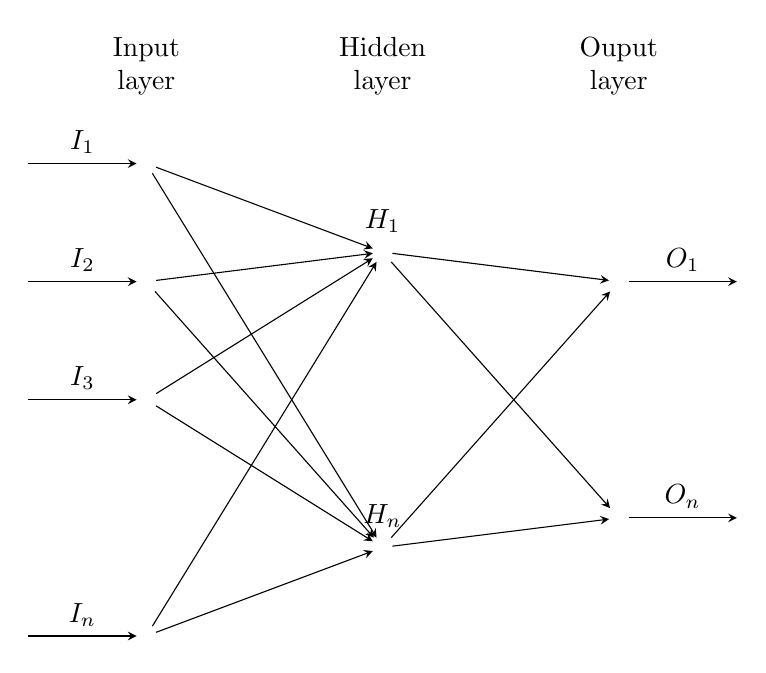
\begin{tikzpicture}[x=1.5cm, y=1.5cm, >=stealth]
	
	\foreach \m/\l [count=\y] in {1,2,3,missing,4}
	\node [every neuron/.try, neuron \m/.try] (input-\m) at (0,2.5-\y) {};
	
	\foreach \m [count=\y] in {1,missing,2}
	\node [every neuron/.try, neuron \m/.try ] (hidden-\m) at (2,2-\y*1.25) {};
	
	\foreach \m [count=\y] in {1,missing,2}
	\node [every neuron/.try, neuron \m/.try ] (output-\m) at (4,1.5-\y) {};
	
	\foreach \l [count=\i] in {1,2,3,n}
	\draw [<-] (input-\i) -- ++(-1,0)
	node [above, midway] {$I_\l$};
	
	\foreach \l [count=\i] in {1,n}
	\node [above] at (hidden-\i.north) {$H_\l$};
	
	\foreach \l [count=\i] in {1,n}
	\draw [->] (output-\i) -- ++(1,0)
	node [above, midway] {$O_\l$};
	
	\foreach \i in {1,...,4}
	\foreach \j in {1,...,2}
	\draw [->] (input-\i) -- (hidden-\j);
	
	\foreach \i in {1,...,2}
	\foreach \j in {1,...,2}
	\draw [->] (hidden-\i) -- (output-\j);
	
	\foreach \l [count=\x from 0] in {Input, Hidden, Ouput}
	\node [align=center, above] at (\x*2,2) {\l \\ layer};
	
	\end{tikzpicture}
\end{minipage}
\fi